\chapter{Einleitung}

\section{Motivation}

\section{Zielstellung}

\section{Unisens}

Das vom Forschungszentrum Informatik und Institut f\"ur Technik der Informationsverarbeitung der Universit\"at Karlsruhe entwickelte Datenformat Unisens dient der Speicherung und der Dokumentation von Sensordaten.
Es ist konzipiert, Daten verschiedener Sensoren innerhalb eines Datensatzes zu speichern.
Ein Datensatz ist im Dateisystem durch ein eigenes Verzeichnis und eine Headerdatei \verb|unisens.xml| hinterlegt.
In der Headerdatei werden alle Informationen \"uber die Bestandteile des Datensatzes, deren Formatierung und ihre semantischen Zusammenh\"ange gespeichert.
Messwerte eines Sensors werden \"ublicherweise in einer Datendatei innerhalb des Verzeichnisses abgespeichert.
Eine solche Datendatei wird als \emph{Entry} in dem Datensatz bezeichnet.
Alle Metainformationen zu den Sensordaten werden in der Headerdatei abgspeichert, so dass die Datendateien immer nur die reinen Messdaten enthalten.
Als m\"ogliche Sensordaten werden sowohl kontinuierlich abgetastete Signale als auch ereignisorientierte Daten unterst\"utzt.
Unisens unterscheidet zwischen vier Arten von Daten:
\begin{description}
	\item[Signale \emph{(Signal)}] \hfill \\
		Signale sind kontinuierlich abgetastete, numerische Messdaten.
		Sie zeichnen sich durch eine beliebige aber konstante Abtastrate und ihre Abtastaufl\"osung aus.
		Zudem k\"onnen Signale aus mehreren Kan\"alen bestehen, die aber alle in ein und derselben Datei abgespeichert werden.
	\item[Ereignisse \emph{(Event)}] \hfill \\
		Ereignisse sind diskrete Zeitpunkte die mit einem textlichen Beschreibung versehen sind. (z.B. Triggersignale)
		Sie zeichnen sich durch einen Zeitstempel und einer kurzen Beschreibung aus.
		Optional k\"onnen noch Kommentare zu einem Ereignis hinzugef\"ugt werden.
	\item[Einzelwerte \emph{(Value)}] \hfill \\
		Einzelwerte sind eine Kombination der beiden oben genannten Datenarten.
		Sie beinhalten numerische Werte die zu bestimmten Zeitpunkten aufgenommen wurden.
		Mit ihnen ist es m\"oglich Daten zu speichern, die nicht in festen Zeitintervallen gemessen werden.
	\item[Propriet\"are Daten \emph{(Custom data)}] \hfill \\
		Mit dieser Art k\"onnen anwendungsspezifisch Daten gespeichert werden, die durch die drei oben genannten Arten nicht erfasst werden k\"onnen.
\end{description}

\subsection{Implementierungsdetails}

In diesem Abschnitt wird kurz auf einige Details der Umsetzung des Unisens-Formates eingegangen.
Unisens ist in Java implementiert und wird unter der \emph{\ac{LGPL}} zur Verf\"ugung gestellt.
Die bereit gestellte Bibliothek ist auf zwei Einzeldateien aufgeteilt: \verb|org.unisens.jar| und \verb|org.unisens.ri.jar|.
Bei der ersten Datei handelt es sich nur um die Definition der Schnittstellen der einzelnen Klassen.
Die eigentliche Umsetzung der Funktionalit\"at ist in der zweiten Datei abgespeichert und die Klassennamen sind durch den Suffix "`Impl"' erweitert.
Eine \"Ubersicht der Klassenstruktur und der von au\ss en ersichtlichen Attribute ist in Abbildung \ref{pic:unisens_interface} dargestellt.

\begin{figure}
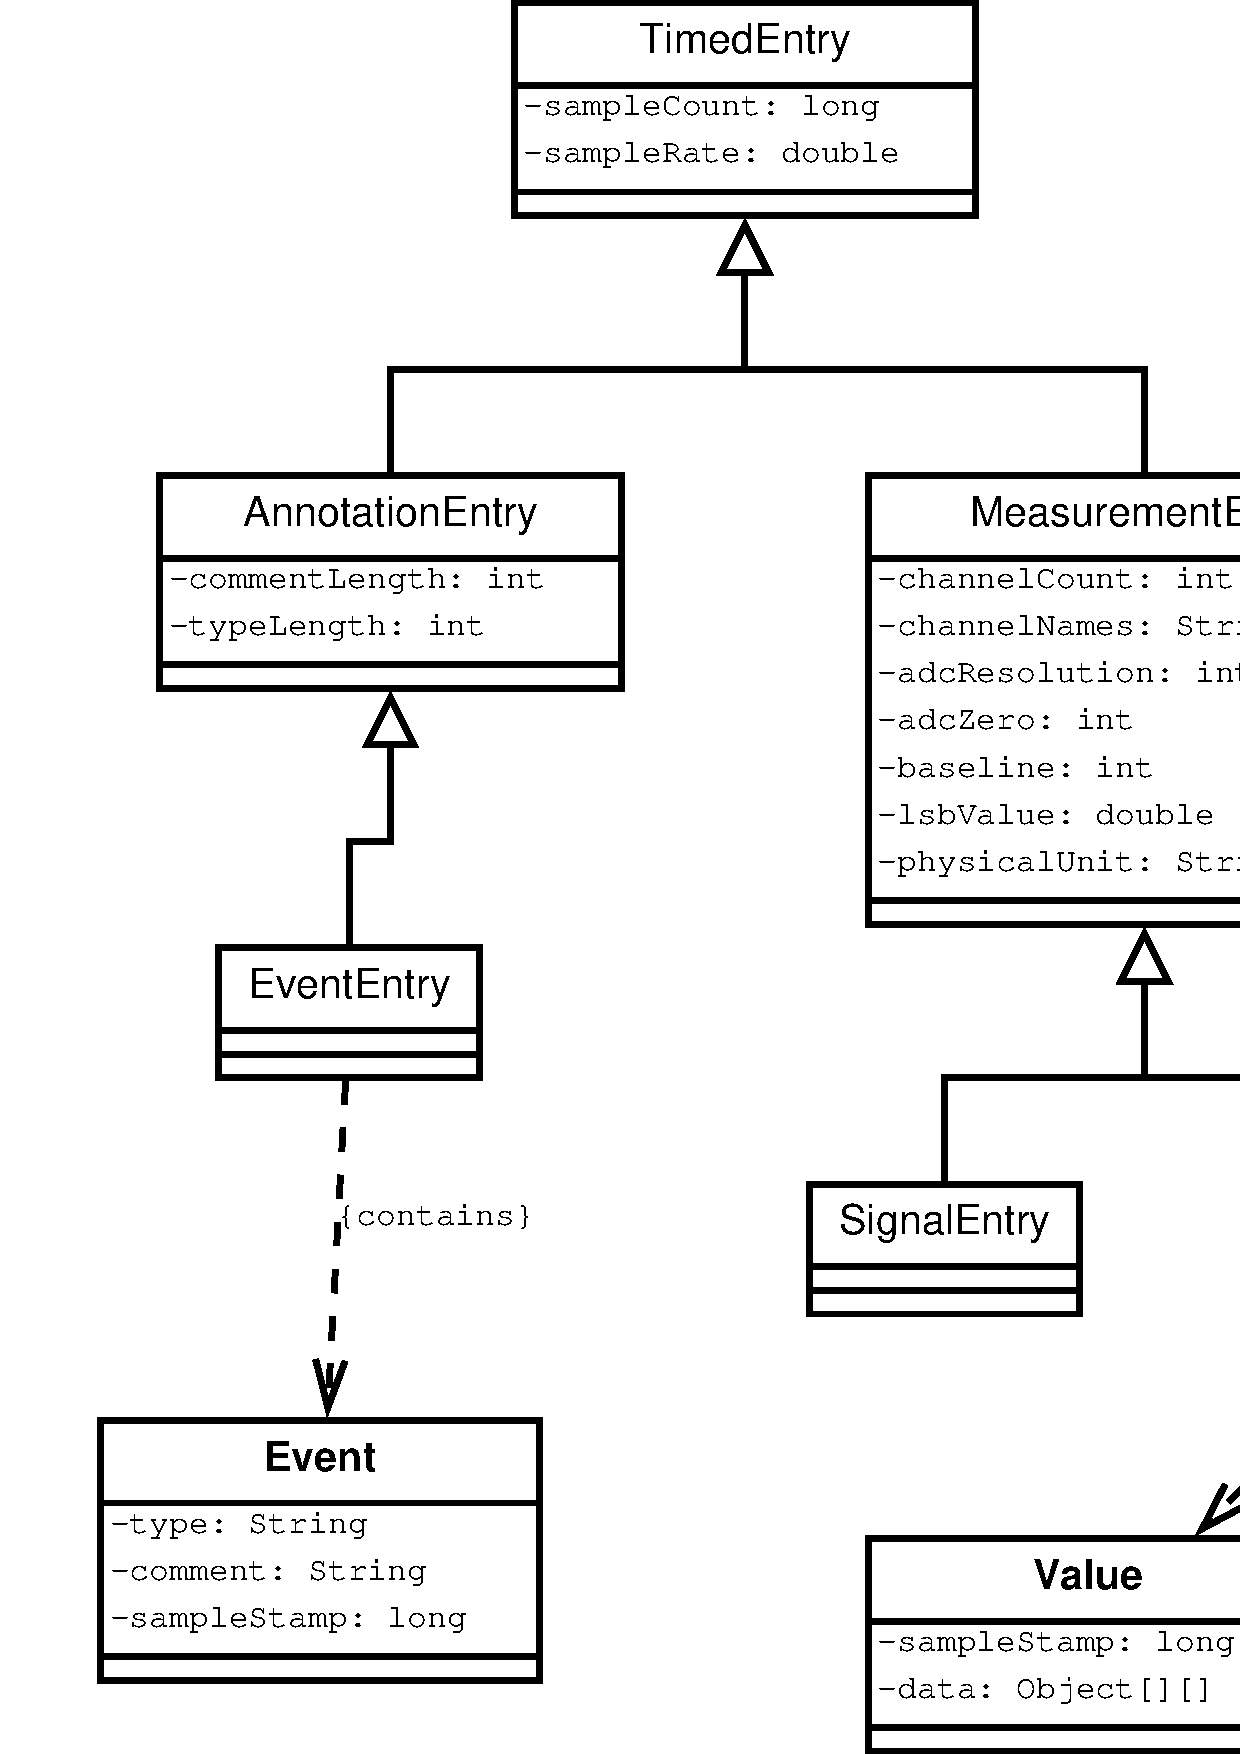
\includegraphics[width=\textwidth]{bilder/unisens_interface.png}
\caption{Klassen\"ubersicht der von Unisens definierten Schnittstellen}
\label{pic:unisens_interface}
\end{figure}

Die Zeitpunkte von Ereignisdaten und Einzelwertdaten werden \"uber eine virtuelle Abtastrate bestimmt.
Der Zeitpunkt eins jeden \emph{Event}- oder \emph{Value}-Eintrags ist als ganzzahlige Samplenummer dieser Abtastrate gespeichert.
Die Zeit eines Ereignisses, relativ zum Messbeginn, errechnet sich somit $Zeitpunkt = {Samplenummer \over Abtastrate}$.
M\"ochte man die M\"oglichkeit Ereignisse f\"ur jeden beliebigen Datenpunkt eines Datensatzes zuordnen zu k\"onnen, dann muss die virtuelle Abtastrate als das kleinste gemeinsame Vielfache aller vorhandenen Abtastraten gew\"ahlt werden.

...

%% EOF %%%%%%%%%%%%%%%%%%%%%%%%%%%%%%%%%%%%%%%%%%%%%%%%%%%%%%
